\documentclass[11pt, a4paper]{article}

% ==========================================
% Preamble & Package Imports
% ==========================================
% Inherit your existing comprehensive thesis preamble
% ***************************************************
% LaTeX Packages
% ***************************************************
% This file defines the document design.
% Usually it is not necessary to edit this file, but you can use it to change aspects of the design if you want.

%There are essential packages that are contained within the StylesAndSettings/uqthesis.cls which are integral to the template - These must not be deleted.

%The packages below are optional, please add or alter as required.

\usepackage[utf8]{inputenc}
\usepackage[T1]{fontenc}
\usepackage{microtype}
\usepackage{bm}
\usepackage{upgreek}
\usepackage{dsfont}
\usepackage{eucal}
\usepackage{stmaryrd}
\usepackage{pifont}
\usepackage{marvosym}
\usepackage{blindtext}
\usepackage{lipsum}
\usepackage{amsmath}
\usepackage{amssymb}
\usepackage{amsthm}
\usepackage{mathtools}
\usepackage{mathdots}
\usepackage{simplewick}
\usepackage{cancel}
\usepackage{siunitx}
\usepackage{nicefrac}
\usepackage[table,dvipsnames]{xcolor}
\definecolor{airforceblue}{RGB}{93,138,168}
\definecolor{darkblue}{rgb}{0.0,0.0,0.55}
\definecolor{cream}{rgb}{1.0,0.99,0.82}
\definecolor{islamicgreen}{rgb}{0.0,0.56,0.0}
\definecolor{thmcolor}{rgb}{0.96,0.92,0.86}
\definecolor{defncolor}{rgb}{0.93,0.96,0.98}
\definecolor{tipcolor}{rgb}{0.94,0.97,0.94}
\definecolor{warncolor}{rgb}{0.98,0.94,0.94}
\definecolor{corcolor}{rgb}{0.96,0.94,0.98}
\definecolor{packcol}{rgb}{0.09,0.45,0.27}
\definecolor{methcol}{rgb}{0.16,0.32,0.75}
\usepackage{graphicx}
\usepackage{transparent}
\usepackage{tikz}
\usepackage{pgfplots}
\usepackage[all]{xy}
\pgfplotsset{compat=1.18}
\usepgfplotslibrary{fillbetween}
\usetikzlibrary{matrix,calc,positioning,arrows.meta,intersections,chains,shapes.geometric,patterns,fpu}
\usepackage{geometry}
\usepackage{fancyhdr}
\usepackage{titlesec}
\usepackage{caption}
\usepackage{subcaption}
\usepackage{float}
\usepackage{placeins}
\usepackage{wrapfig}
\usepackage{rotating}
\usepackage{chngcntr}
\usepackage{pdfpages}
\usepackage{setspace}
\usepackage{multicol}
\usepackage{multirow}
\usepackage{dcolumn}
\usepackage{varwidth}
\usepackage{booktabs}
\usepackage{ragged2e}
\usepackage{array}
\usepackage{enumerate}
\usepackage{mdwlist}
\usepackage{framed}
\usepackage{mdframed}
\usepackage[most]{tcolorbox}
\tcbuselibrary{skins,breakable,theorems,listings}
\usepackage{algorithm}
\usepackage{algpseudocode}
\numberwithin{algorithm}{section}
\usepackage{cite}
\usepackage{hyperref}
\usepackage[nameinlink]{cleveref}

\hypersetup{
	colorlinks=true,
	linkcolor=darkblue,
	citecolor=darkblue,
	urlcolor=darkblue,
	breaklinks=true
}

\theoremstyle{definition}
\newtheorem{definition}{Definition}[section]
\newtheorem{condition}{Condition}[section]

\theoremstyle{plain}
\newtheorem{theorem}{Theorem}[section]
\newtheorem{lemma}{Lemma}[section]

%This defines some macros that implement Latin abbreviations

\newcommand{\via}{\textit{via}} %Italicised via.
\newcommand{\ie}{\textit{i.e.}} %Literally.
\newcommand{\eg}{\textit{e.g.}} %For example.
\newcommand{\etc}{\textit{etc.}} %So on...
\newcommand{\vv}{\textit{vice versa}} %And the other way around.
\newcommand{\viz}{\textit{viz}.} %Resulting in.
\newcommand{\cf}{\textit{cf}.} %See, or 'consistent with'.
\newcommand{\apr}{\textit{a priori}} %Before the fact.
\newcommand{\apo}{\textit{a posteriori}} %After the fact.
\newcommand{\vivo}{\textit{in vivo}} %In the flesh.
\newcommand{\situ}{\textit{in situ}} %On location.
\newcommand{\silico}{\textit{in silico}} %Simulation.
\newcommand{\vitro}{\textit{in vitro}} %In glass.
\newcommand{\vs}{\textit{versus}} %James \vs{} Pete.
\newcommand{\ala}{\textit{\`{a} la}} %In the manner of...
\newcommand{\apriori}{\textit{a priori}} %Before hand.
\newcommand{\etal}{\textit{et al.}} %And others, with correct punctuation.
\newcommand{\naive}{na\"\i{}ve} %Queen Amidala is young and \naive{}.

\DeclarePairedDelimiter\abs{\lvert}{\rvert}
\DeclarePairedDelimiter\norm{\lVert}{\rVert}
\DeclarePairedDelimiter\set{\{}{\}}
\DeclarePairedDelimiter\ceil{\lceil}{\rceil}
\DeclarePairedDelimiter\floor{\lfloor}{\rfloor}
\DeclarePairedDelimiterX\inner[2]{\langle}{\rangle}{#1, #2}

\providecommand{\mathdefault}[1]{#1}

\newcommand{\R}{\mathbb{R}}
\newcommand{\N}{\mathbb{N}}
\newcommand{\Z}{\mathbb{Z}}
\newcommand{\C}{\mathbb{C}}
\newcommand{\Prob}{\mathbb{P}}
\newcommand{\gvn}{\mid}  % "given" in conditional probability, e.g. P(A \gvn B)
\newcommand{\matX}{\mathcal{X}}  % state space (e.g. $\matX \subseteq \R^n$)
\newcommand{\E}{\mathbb{E}}
\newcommand{\Var}{\mathrm{Var}}
\newcommand{\Cov}{\mathrm{Cov}}
\newcommand{\tr}{\mathrm{tr}}
\newcommand{\indsim}{\stackrel{\mathrm{ind}}{\sim}}
\newcommand{\iidsim}{\stackrel{\mathrm{iid}}{\sim}}
\newcommand{\la}{\leftarrow}
% Distribution names (for notation tables / "X \sim \Ber(p)")
\newcommand{\Ber}{\mathrm{Ber}}
\newcommand{\Bin}{\mathrm{Bin}}
\newcommand{\Exp}{\mathrm{Exp}}
\newcommand{\Gam}{\mathrm{Gamma}}
\newcommand{\Geo}{\mathrm{Geo}}
\newcommand{\Nor}{\mathcal{N}}
\newcommand{\Poi}{\mathrm{Po}}
\newcommand{\Unif}{\mathrm{Unif}}

\newcommand{\bx}{\boldsymbol{x}}
\newcommand{\by}{\boldsymbol{y}}
\newcommand{\bz}{\boldsymbol{z}}
\newcommand{\btheta}{\boldsymbol{\theta}}
\newcommand{\bmu}{\boldsymbol{\mu}}
\newcommand{\bSigma}{\boldsymbol{\Sigma}}
\newcommand{\bX}{\boldsymbol{X}}
\newcommand{\bW}{\boldsymbol{W}}


% Define Official UQ Brand Colors for Heading Styling
\definecolor{uqpurple}{RGB}{81,36,122}

% Customize Section Headings
\titleformat{\section}{\Large\bfseries\color{uqpurple}}{\thesection}{1em}{}
\titleformat{\subsection}{\large\bfseries\color{darkblue}}{\thesubsection}{1em}{}

% Paragraph Formatting
\onehalfspacing
\setlength{\parindent}{0pt}
\setlength{\parskip}{1em}

% ==========================================
% Title Block
% ==========================================
\title{\vspace{-2cm}\textbf{\color{uqpurple}RBUS6923 Workshop Critique}\\ \Large Beyond Representation: Diversity, Interpersonal Distance, and Information Access in Corporate Boards}
\author{\textbf{Zac Kienzle} \\ The University of Queensland}
\date{\today}

\begin{document}

\maketitle
\vspace{-1cm}
\rule{\textwidth}{0.4pt}
\vspace{0.5cm}

% ==========================================
% Step #1: 'Front End'
% ==========================================
\section*{Step \#1: 'Front End'}

\subsection*{Motivation and Fit with Extant Literature}
The manuscript investigates whether the aggregate interpersonal distance between a director and their peers inhibits their access to the board's informal information sharing network. This is a highly important and timely governance issue. It shifts the academic focus from structural demographic quotas to the operational reality of cognitive integration and information flow within corporate hierarchies.

The paper successfully challenges the naive inductivist approaches prevalent in prior diversity literature, which typically isolate single demographic traits like gender or ethnicity to predict board performance. By leveraging theories of group dynamics and homophily, the authors introduce a compelling theoretical tension. Regulatory mandates universally promote diverse representation under the assumption that it automatically yields diverse cognitive input. The authors present a falsifiable conjecture proposing the exact opposite outcome: high interpersonal distance triggers subgroup factionalism and excludes diverse directors from the private information network, thereby neutralizing the intended benefits of representation.

\subsection*{Formalisation of Hypotheses and Conceptual Foundation}
The conceptual foundation is robustly grounded in resource dependence theory and social distance theory. The authors formulate a bold, risky conjecture in the Popperian sense \cite{popper_logic_2005}. They hypothesize that highly unique directors suffer a measurable informational penalty, which can be observed empirically through their disadvantaged insider trading behavior relative to their tightly integrated peers.

\subsection*{Ex Ante Potential Contribution}
The ex ante potential contribution is substantial. By reframing the debate from structural representation to behavioral interaction and information flow, the study offers a novel mechanism to explain the mixed governance outcomes associated with diversity initiatives. The anticipated findings are highly uncertain prior to empirical testing, confirming the presence of genuine theoretical tension that meaningfully informs a gap in current knowledge.

% ==========================================
% Step #2: Methodology / Experimental Design
% ==========================================
\section*{Step \#2: Methodology / Experimental Design}

\subsection*{Approach and Construct Validity}
The linkage between the theoretical constructs and operational proxies demonstrates rigorous design alongside measurable slippage. The independent variable is operationalized using a Mahalanobis distance metric calculated across 17 functional and demographic characteristics. This elegant methodological choice successfully captures the multidimensionality of perceived interpersonal difference while mathematically correcting for covariance among professional traits.

Conversely, the dependent variable carries a moderate threat to construct validity. Utilizing open-market share purchases and trade timing as proxies for informational inclusion involves inherent assumptions. Distant directors might simply possess different capital constraints, distinct risk tolerances, or stricter ethical interpretations of their governance roles, rather than lacking access to the information entirely.

\subsection*{Internal Validity}
The research design meticulously attempts to isolate the primary effect by turning only one dial. The authors mitigate alternative explanations by employing firm and year fixed effects to control for unobservable, time-invariant corporate characteristics and macroeconomic shifts. Crucially, the model includes controls for direct social ties to executives and other independent directors, separating structural homophily from pre-existing interpersonal networking.

Despite these robust controls, dynamic endogeneity remains a latent threat. Unobservable, time-varying corporate culture could simultaneously drive the appointment of distant window-dressing directors and foster opaque internal information environments.

\begin{figure}[H]
	\centering
	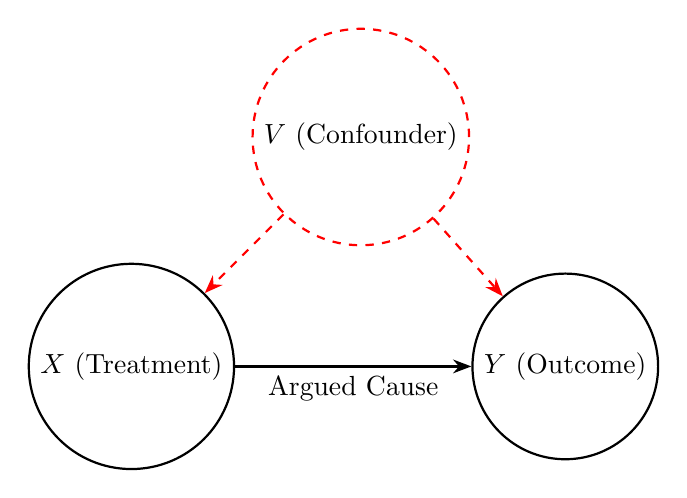
\begin{tikzpicture}[
			node distance=2cm and 3cm,
			>=Stealth,
			main/.style={circle, draw, minimum size=1cm, thick},
			confound/.style={circle, draw=red, minimum size=1cm, thick, dashed}
		]
		% Nodes
		\node[main] (X) {$X$ (Treatment)};
		\node[main] (Y) [right=of X] {$Y$ (Outcome)};
		\node[confound] (V) [above right=1cm and 1cm of X] {$V$ (Confounder)};

		% Arrows
		\draw[->, thick] (X) -- node[below] {Argued Cause} (Y);
		\draw[->, thick, dashed, red] (V) -- (X);
		\draw[->, thick, dashed, red] (V) -- (Y);
	\end{tikzpicture}
	\caption{Threat to Internal Validity: Dynamic endogeneity ($V$) driving both director distance ($X$) and information access ($Y$).}
\end{figure}

\subsection*{Statistical Analysis Validity}
The statistical validity of the study is exceptional. The researchers utilize a massive and highly representative sample of 50,712 observations spanning two decades. This yields immense statistical power, effectively minimizing the risk of Type II errors. Furthermore, the authors appropriately address cross-sectional and time-series dependence within their panel data by clustering standard errors at the firm and year levels.

\begin{equation}
	Y_{it} = \beta_0 + \beta_1 \mathit{Distance}_{it} + \bm{\gamma}^{\top} \bX_{it} + \alpha_i + \delta_t + \varepsilon_{it}
\end{equation}

\begin{table}[H]
	\centering
	\caption{Demonstration of OLS Regression Results}
	\vspace{0.2cm}
	\begin{tabular}{l c c}
		\toprule
		\textbf{Variables} & \textbf{Model 1} & \textbf{Model 2} \\
		\midrule
		Distance ($X$)     & -0.112***        & -0.089**         \\
		                   & (0.039)          & (0.041)          \\
		Firm Size ($V$)    &                  & 0.045***         \\
		                   &                  & (0.012)          \\
		\midrule
		Observations       & 50,712           & 50,712           \\
		Adjusted $R^2$     & 0.264            & 0.366            \\
		Firm \& Year FE    & Yes              & Yes              \\
		\bottomrule
	\end{tabular}
\end{table}

% ==========================================
% Step #3: Findings and Conclusions
% ==========================================
\section*{Step \#3: Findings and Conclusions ('Accomplishments')}

\subsection*{Significance of Findings}
The empirical results achieve high statistical significance and profound economic materiality. A one standard deviation increase in interpersonal distance yields a 1.92 percent reduction in abnormal returns over a 180-day window. The authors note this translates to a 38.64 percent relative decrease compared to the baseline independent director return. This constitutes a massive economic penalty for unintegrated directors.

\subsection*{Plausibility and Fit with Hypotheses}
The findings are highly plausible. The analysis reveals that functional distance drives this exclusion much more powerfully than demographic distance. This aligns perfectly with the professionalized reality of corporate boards, where shared industry experience and financial vocabularies dictate informal integration far more than demographic traits.

The data strictly corroborate the hypothesis that distant directors are excluded from informal networks. The chain timing analysis provides a decisive corroboration. It demonstrates that distant directors mechanically rely on public SEC Form 4 disclosures to trigger their trades rather than engaging in the private, concurrent trade coordination enjoyed by their integrated peers.

\subsection*{External Validity (Generalisability)}
The external validity is inherently constrained by the institutional setting. The reliance on Form 4 filings isolates the sample entirely to US public firms operating under strict SEC regulatory environments. These specific homophilic information dynamics may not generalize to international jurisdictions with divergent governance traditions, such as the two-tier supervisory boards prevalent in the European corporate economy.

% ==========================================
% Overall Summary Assessment
% ==========================================
\section*{Overall Summary Assessment}
This manuscript represents a highly credible and pedagogically efficient demonstration of empirical accounting research. The front end establishes a compelling theoretical tension that moves beyond isolated trait analysis. The methodology exhibits exceptional internal and statistical validity, successfully navigating the construct slippage inherent in utilizing insider trading as an information proxy. The accomplishments are economically material and theoretically cohesive. Ultimately, the study delivers a significant contribution to the literature by empirically proving that granting a diverse director structural representation does not guarantee them integration into the board's private informational discourse.

\bibliographystyle{StylesAndSettings/abbrv-unsrt}
\bibliography{References/References}

\end{document}
